\section{Solution}

\subsection{Classification}
In this competition, since the data is organized in a time-series format, it is
intuitive to represent the data using the Hidden Markov Model~\cite{HMM1996}
which is a generative probabilistic model, in which a sequence of observable
variables (which in our case, is the X, Y, Z coordinate) is generated by a
sequence of internal hidden states.

In this dataset, we postulate that each hidden state should correspond to the
activity that the users are currently carrying out such as running, walking and
so on. However, it is hard for us to model what will be the possible different
activities of each user as there is no data related to the user activity. 
Having too many states will cause an overfit for our
training set while too few states will cause an underfit. To that end, we
perform a limited exhaustive enumeration of the hidden states to compute the
optimal performance.

Additionally, for each of the mobile users, there will be certain phone
position in which the user will have the phone under. At some time, the users
might shake the phones slightly while at rarer times, the users might move the
phones much faster and the X,Y,Z values are continuous variables.
Thus, we model our observable variables as Gaussian variables. The HMM
is learned by using an iterative Expectation-Maximization (EM) algorithm, 
Baum-Welch~\cite{BaumWelch}.

\begin{figure}[h]
  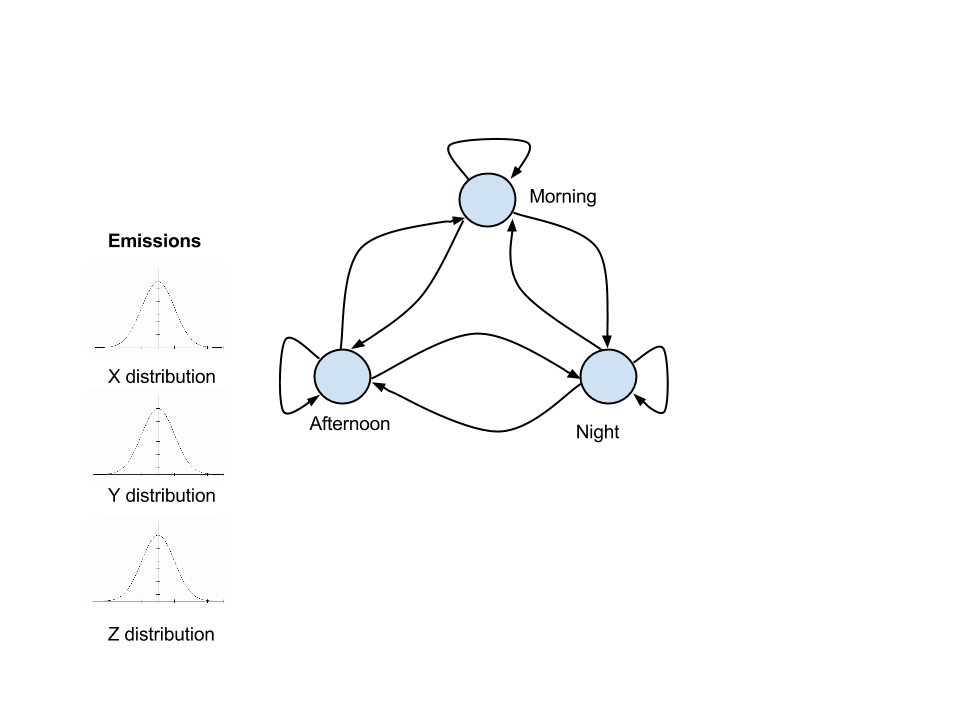
\includegraphics[width=\linewidth]{./figs/HMM.png}
  \label{fig:points}
\end{figure}

Our next insight is that although for each user there will be a certain
coordinate that is "popular" with a particular user, there will be other coordinates
that will also be "popular" for the user. To account for such possibilities, we
model each of our coordinate as a Gaussian mixtures~\cite{GMM2009}. Again, it
is impossible to evaluate what will be the optimal number of Gaussian mixtures
to model a coordinate which we then resort (again) to a limited exhaustive
enumeration. Similarly, the HMM is learned with the Baum-Welch algorithm~\cite{BaumWelch}.

Finally, due to the time-series nature of the data, we postulate that we could
perform k-fold cross-validation~\cite{KFold2013} in which the data set is
divided into k consecutive subsets (i.e. no shuffling), and then we perform
cross-validation method k times. Each time, one of the k subsets is being left
out and the other k-1 subsets are put together to form a training set. For our
purpose, we build k HMM model and each of the questions is then being evaluated
against these models.

Incorporating the above insights to our model has yielded a \textbf{79.4\%}
classification accuracy on the Kaggle leaderboard.

\subsection{Clustering}
In the previous section, we knew which device id we needed the test sequence
to compare to. If this information was not available to us, we would need
to do a linear scan through every device in the training set for every
test sequence. Hence, the runtime is \textit{O}($nm$) where $n$ is the
number of device ids and $m$ the number of test sequences. With our
training and test data files, it took us ~15 hours to do classification.

An interesting sub-problem would be to find a cheap and efficient way of
doing search space reduction. We decided to apply the k-means clustering
algorithm~\cite{kmeans} to create $\sqrt{387} \simeq 20$ clusters, and only build HMMs
after finding which cluster the sequence is most likely part of. We used both
euclidian distance and cosine similarity as our distance measures between
clusters.

\begin{program}
\mbox{\textit{\textbf{k-means(devices, k)}}}
\BEGIN \\
  samples := randomsample(devices, k) \\
  clusters := [] \\
  \FOR sample <- samples \DO
    clusters.add([sample]) \OD
  means := findmeans(clusters)
  \WHILE is\ not\ converged(clusters) \DO
    clusters := [[]\ for\ k]
    \FOR device <- devices \DO
      \FOR i <- 0..k \DO
        m = means[i]
        d = distance(device, m)
        \IF is\ best\ distance(d)
          clusters[i].add(device)
        \OD
        \OD
    means = findmeans(clusters)
    \OD
\END
\end{program}
The distance() function can be implemented with euclidian distance. In this
situation, we observe that the sizes of our clusters are very skewed.

\begin{figure}[H]
  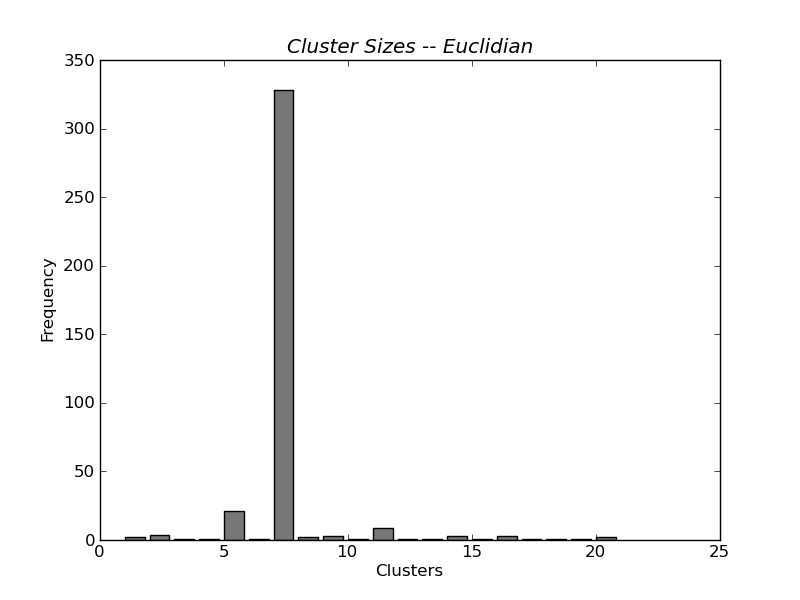
\includegraphics[width=\linewidth]{./figs/euclidian.png}
  \label{fig:euclidian}
\end{figure}

However, if we use cosine similarity as a distance measurements we get even
cluster sizes. Therefore, it is preferable to use cosine similarity as
the distance measurement.

\begin{figure}[H]
  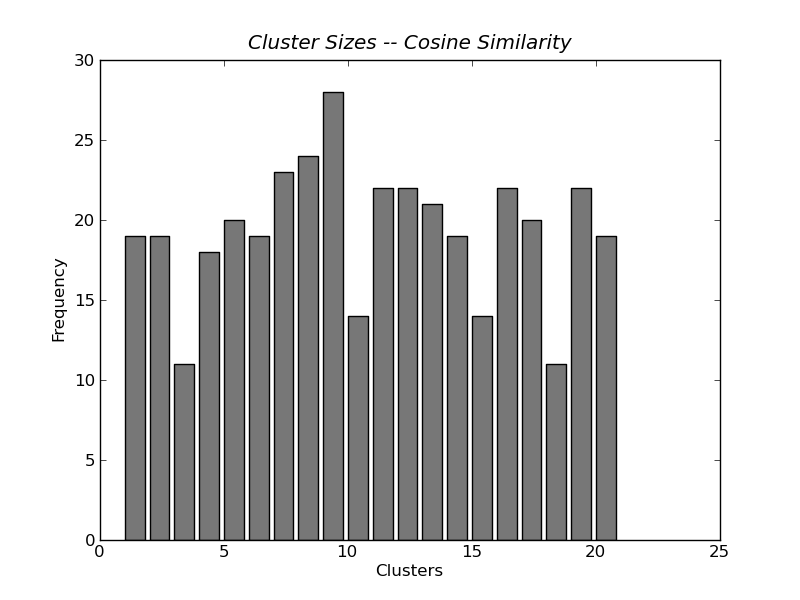
\includegraphics[width=\linewidth]{./figs/cosine.png}
  \label{fig:cosine}
\end{figure}

Lastly, we went through the test sequences and applied cosine similarity between
the sequences and the mean of each cluster to find which one is the closest. However,
the accuracy of finding the correct cluster was surprisingly low, at $5.7\%$. This is only
$0.7\%$ better than assigning at random to a cluster. We decided to visualize our clusters
to get an insight to this problem.

\begin{figure}[H]
  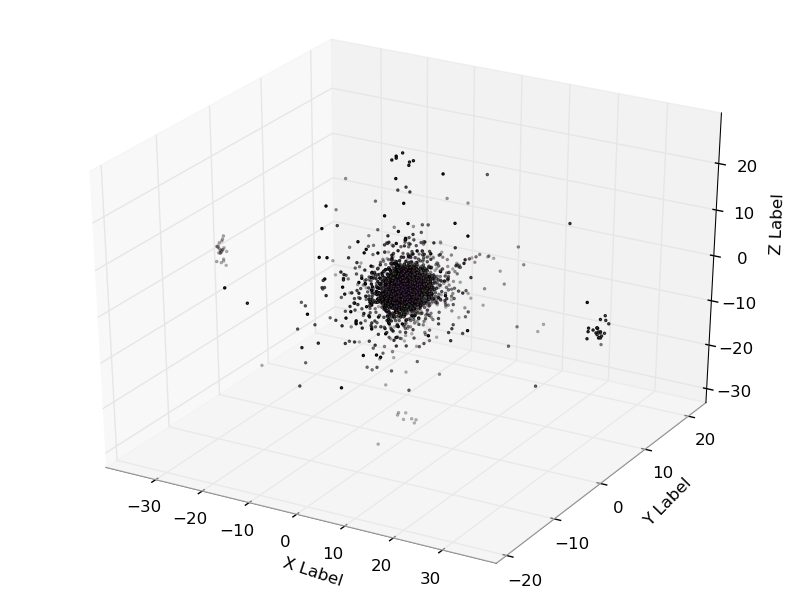
\includegraphics[width=\linewidth]{./figs/points.png}
  \label{fig:points}
\end{figure}

This figure explains why we get low accuracy, as all the data points are really close to each
other it is very difficult to separate it into well-defined clusters. Therefore, the observation
of skewed data for the euclidian distance heuristic makes sense as all the points near (0,0,0) 
are in the same cluster except few outliers.

We could use the euclidian heuristic instead of cosine similarity which will allow us to reach 
much higher accuracy as we will have more than 300 devices in the same cluster but then we lose the
point of pruning the search space.
